\documentclass[aspectratio=169,11pt]{beamer}

\usetheme{Madrid}
\usecolortheme{default}
\setbeamertemplate{navigation symbols}{}
\setbeamertemplate{footline}[frame number]

\usepackage[T1]{fontenc}
\usepackage[utf8]{inputenc}
\usepackage{lmodern}
\usepackage{amsmath}
\usepackage{amssymb}
\usepackage{booktabs}
\usepackage{tabularx}
\usepackage{tikz}
\usepackage{listings}
\usepackage{xcolor}
\usepackage{pgfplots}
\pgfplotsset{compat=1.16}
\usetikzlibrary{positioning, arrows.meta}

\definecolor{sdmblue}{RGB}{27, 74, 125}
\definecolor{sdmteal}{RGB}{0, 130, 127}
\definecolor{sdmorange}{RGB}{222, 123, 35}
\definecolor{sdmlight}{RGB}{244, 247, 250}
\definecolor{sdmgreen}{RGB}{67, 142, 75}
\definecolor{sdmred}{RGB}{195, 64, 64}
\definecolor{codebg}{RGB}{247, 248, 250}

\setbeamercolor{structure}{fg=sdmblue}
\setbeamercolor{palette primary}{bg=sdmblue, fg=white}
\setbeamercolor{palette secondary}{bg=sdmteal, fg=white}
\setbeamercolor{palette tertiary}{bg=sdmblue, fg=white}
\setbeamercolor{title}{fg=sdmblue}
\setbeamercolor{frametitle}{bg=sdmblue!8, fg=sdmblue}
\setbeamercolor{block title}{bg=sdmblue, fg=white}
\setbeamercolor{block body}{bg=sdmlight, fg=black}
\setbeamercolor{alerted text}{fg=sdmorange}

\lstset{
  basicstyle=\ttfamily\scriptsize,
  backgroundcolor=\color{codebg},
  frame=single,
  rulecolor=\color{sdmblue!30},
  columns=fullflexible,
  keepspaces=true,
  showstringspaces=false,
  breaklines=true
}

\title{Phased Fine-Tuning of POMO with Three Inductive-Bias Modules}
\subtitle{SDM-5031 Course Project --- Spring 2026}
\author{[Your Name]}
\date{\today}

\begin{document}

% =====================================================================
% Slide 1: Title
% =====================================================================
\begin{frame}[plain]
  \vspace{0.5cm}
  {\usebeamerfont{title}\color{sdmblue}\LARGE\textbf{Phased Fine-Tuning of POMO}\par}
  \vspace{0.1cm}
  {\usebeamerfont{title}\color{sdmblue}\Large\textbf{with Three Inductive-Bias Modules for TSP}\par}
  \vspace{0.6cm}
  {\large SDM-5031 Course Project --- Spring 2026\par}
  \vspace{0.4cm}
  {[Your Name]\par}

  \vspace{1.0cm}
  \begin{columns}[T,totalwidth=\textwidth]
    \begin{column}{0.55\textwidth}
      \begin{block}{Headline result}
        \textbf{51.8\%} relative reduction in \texttt{avg\_aug\_gap}
        on the validation set, starting from the bundled
        3000-epoch POMO baseline with only 400 extra fine-tune epochs.
      \end{block}
    \end{column}
    \begin{column}{0.40\textwidth}
      \begin{alertblock}{Three modules}
        \begin{itemize}
          \item M2: distance / kNN logit bias
          \item MSC: structured curriculum data
          \item M3: leader-focused reward
        \end{itemize}
      \end{alertblock}
    \end{column}
  \end{columns}
  \vfill
\end{frame}

% =====================================================================
% Slide 2: Problem & Motivation
% =====================================================================
\begin{frame}{TSP, POMO Baseline, and Where We Improve}
  \begin{columns}[T,totalwidth=\textwidth]
    \begin{column}{0.55\textwidth}
      \begin{block}{Setup}
        \begin{itemize}
          \item TSP is NP-hard; POMO trains a Transformer policy on TSP-100
                with multi-rollout REINFORCE
          \item Course gives a 3000-epoch baseline checkpoint
          \item Budget: \textbf{400 extra fine-tune epochs}
          \item Official metric: \texttt{avg\_aug\_gap}
                (best across 8-fold augmentation)
        \end{itemize}
      \end{block}
      \begin{block}{Why this is non-trivial}
        Naive 400-epoch fine-tune barely moves the needle ---
        the baseline is already converged on uniform $[0,1]^2$ data.
      \end{block}
    \end{column}
    \begin{column}{0.42\textwidth}
      \centering
      \begin{tabular}{lc}
        \toprule
        \textbf{Setting} & \textbf{val \texttt{avg\_aug\_gap}} \\
        \midrule
        Baseline (3000 ep) & 2.330\% \\
        +400 ep, no modules & 1.962\% \\
        \rowcolor{sdmblue!12}
        \textbf{+400 ep, three modules} & \textbf{1.122\%} \\
        \bottomrule
      \end{tabular}
      \vspace{0.4cm}

      {\color{sdmorange}\textbf{Pure fine-tune buys 0.37\%.}}\\
      {\color{sdmblue}\textbf{Modules buy another 0.84\%.}}
    \end{column}
  \end{columns}
\end{frame}

% =====================================================================
% Slide 3: Three Innovations Overview
% =====================================================================
\begin{frame}{Three Modules at Three Levels of the Pipeline}
  \centering
  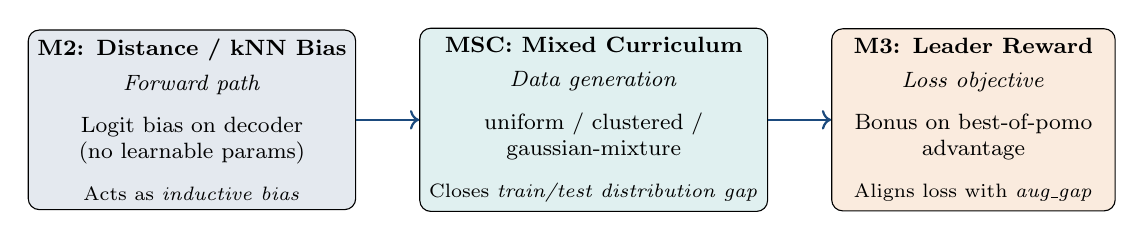
\begin{tikzpicture}[node distance=0.8cm, every node/.style={align=center, font=\footnotesize}]
    \node[draw, rounded corners, fill=sdmblue!12, minimum width=3.6cm, minimum height=2.2cm] (m2)
      {\textbf{M2: Distance / kNN Bias}\\[0.1cm]
       \textit{Forward path}\\[0.2cm]
       Logit bias on decoder\\
       (no learnable params)\\[0.2cm]
       \scriptsize Acts as \emph{inductive bias}};

    \node[draw, rounded corners, fill=sdmteal!12, minimum width=3.6cm, minimum height=2.2cm, right=of m2] (msc)
      {\textbf{MSC: Mixed Curriculum}\\[0.1cm]
       \textit{Data generation}\\[0.2cm]
       uniform / clustered /\\
       gaussian-mixture\\[0.2cm]
       \scriptsize Closes \emph{train/test distribution gap}};

    \node[draw, rounded corners, fill=sdmorange!15, minimum width=3.6cm, minimum height=2.2cm, right=of msc] (m3)
      {\textbf{M3: Leader Reward}\\[0.1cm]
       \textit{Loss objective}\\[0.2cm]
       Bonus on best-of-pomo\\
       advantage\\[0.2cm]
       \scriptsize Aligns loss with \emph{aug\_gap}};

    \draw[->, thick, sdmblue] (m2) -- (msc);
    \draw[->, thick, sdmblue] (msc) -- (m3);
  \end{tikzpicture}

  \vspace{0.6cm}
  \begin{alertblock}{Design principle}
    Each module acts on a \textbf{different level} of the pipeline.
    They can be independently enabled / disabled, which makes ablation clean.
  \end{alertblock}
\end{frame}

% =====================================================================
% Slide 4: M2 Distance/kNN Bias
% =====================================================================
\begin{frame}{M2 --- Distance-Aware / kNN Logit Bias}
  \begin{columns}[T,totalwidth=\textwidth]
    \begin{column}{0.55\textwidth}
      \begin{block}{Mechanism}
        At each decoding step, add a bias to the next-node logit:
        $$
          \ell_{ij} \leftarrow \ell_{ij}
          - \alpha \cdot \tilde{d}_{ij}
          + \beta \cdot \mathbb{1}\!\left[j \in \mathrm{kNN}(i)\right]
        $$
        \begin{itemize}\setlength{\itemsep}{2pt}
          \item $\tilde{d}_{ij}$: mean-normalized Euclidean distance
          \item $\mathrm{kNN}(i)$: $k$ nearest neighbours (raw distance)
          \item $\alpha = \beta = 1.0$, $k = 20$ (swept)
          \item \textbf{Zero learnable parameters}
        \end{itemize}
      \end{block}
    \end{column}
    \begin{column}{0.42\textwidth}
      \begin{block}{Why it helps}
        \begin{itemize}
          \item The encoder gets only $(x, y)$; distance is not an input feature
          \item Bias is a \emph{cheap surrogate} that injects geometric prior at the logit level
          \item Avoids architectural changes (input dim stays 2)
          \item Linear warm-up over Phase 1 prevents disturbing the baseline representation
        \end{itemize}
      \end{block}
      \begin{alertblock}{Engineering detail}
        Bias config is embedded in the saved checkpoint and \textbf{auto-attached at test time} ---
        no extra CLI flag required by the grader.
      \end{alertblock}
    \end{column}
  \end{columns}
\end{frame}

% =====================================================================
% Slide 5: MSC
% =====================================================================
\begin{frame}{MSC --- Mixed Structured Curriculum}
  \begin{columns}[T,totalwidth=\textwidth]
    \begin{column}{0.55\textwidth}
      \begin{block}{Why \texttt{torch.rand()} is not enough}
        Baseline POMO trains on \emph{i.i.d.\ uniform} points in $[0,1]^2$,
        but TSPLIB instances are mostly \emph{structured} (drilling, VLSI, clustered).

        $\Rightarrow$ train / test distribution mismatch hurts generalization.
      \end{block}
      \begin{block}{Three generators, mixed per-batch}
        \begin{itemize}\setlength{\itemsep}{2pt}
          \item \textbf{uniform}: legacy POMO sampler
          \item \textbf{clustered\_uniform}: $K\sim U[3,6]$ Gaussian clusters + small uniform background
          \item \textbf{gaussian\_mixture}: random-weight GMM, all clipped to $[0,1]^2$
        \end{itemize}
      \end{block}
    \end{column}
    \begin{column}{0.42\textwidth}
      \begin{block}{Phase-wise mixing ratios}
        \footnotesize
        \begin{tabularx}{\linewidth}{lccc}
          \toprule
                  & uniform & clustered & gaussian \\
          \midrule
          Phase 1 & 0.6     & 0.3       & 0.1      \\
          Phase 2 & 0.4     & 0.4       & 0.2      \\
          Phase 3 & 0.2     & 0.5       & 0.3      \\
          \bottomrule
        \end{tabularx}
        \vspace{0.2cm}

        Hard distributions are gradually emphasized.
      \end{block}
      \centering
      {\color{sdmblue}\itshape Closes train / test distribution gap on TSPLIB.}
    \end{column}
  \end{columns}
\end{frame}

% =====================================================================
% Slide 6: M3 Leader-focused Reward
% =====================================================================
\begin{frame}{M3 --- Leader-Focused Reward}
  \begin{columns}[T,totalwidth=\textwidth]
    \begin{column}{0.55\textwidth}
      \begin{block}{Aligning loss with the test metric}
        Test metric is \textbf{best-of-pomo} (under 8-fold augmentation),
        but POMO's training advantage is centred at the \emph{mean}:
        $$
          A_i^{\text{POMO}} = r_i - \bar{r}
          \;\;\;\;\;
          \mathcal{L}^{\text{POMO}} = -\mathbb{E}\!\left[A_i \log p_i\right]
        $$
      \end{block}
      \begin{block}{Leader-focused advantage (\texttt{bonus\_adv})}
        $$
          A_i = (r_i - \bar{r}) + \gamma\,(r_{\max} - \bar{r})\cdot
          \mathbb{1}\!\left[i = \arg\max_j r_j\right]
        $$
        \begin{itemize}
          \item $\gamma$ ramps $0 \!\to\! \gamma_0 \!\to\! \gamma_1$ during Phase 3
          \item Higher $\gamma$ emphasizes the best rollout's signal
        \end{itemize}
      \end{block}
    \end{column}
    \begin{column}{0.42\textwidth}
      \begin{block}{Why this matters}
        \begin{itemize}\setlength{\itemsep}{2pt}
          \item Test \texttt{aug\_gap} = $\min$ over 8 augmentations
          \item POMO advantage rewards \emph{average} performance across rollouts
          \item Leader bonus \textbf{shifts gradient} to push the best rollout further
          \item Direct alignment with the evaluation metric
        \end{itemize}
      \end{block}
      \begin{alertblock}{Coupling with lr}
        Phase 3 ramps lr from $1\!\times\!10^{-5}$ to $5\!\times\!10^{-5}$
        (5$\times$ higher) to give the leader signal enough push,
        then decays $10\times$ to $5\!\times\!10^{-6}$.
      \end{alertblock}
    \end{column}
  \end{columns}
\end{frame}

% =====================================================================
% Slide 7: Phased Training Framework
% =====================================================================
\begin{frame}{Phased Schedule --- When to Activate What}
  \centering
  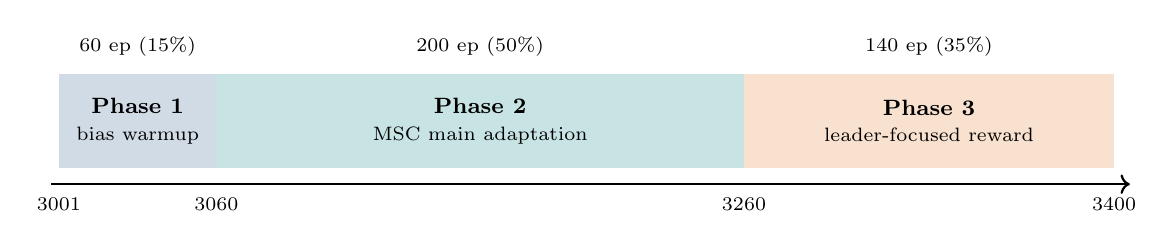
\begin{tikzpicture}[every node/.style={align=center, font=\footnotesize}]
    \fill[sdmblue!20]   (0,0)   rectangle (2.0, 1.2);
    \fill[sdmteal!22]   (2.0,0) rectangle (8.7, 1.2);
    \fill[sdmorange!22] (8.7,0) rectangle (13.4, 1.2);

    \node at (1.0, 0.6)  {\textbf{Phase 1}\\\scriptsize bias warmup};
    \node at (5.35, 0.6) {\textbf{Phase 2}\\\scriptsize MSC main adaptation};
    \node at (11.05, 0.6){\textbf{Phase 3}\\\scriptsize leader-focused reward};

    \draw[->, thick] (-0.1, -0.2) -- (13.6, -0.2);
    \node[anchor=north] at (0.0, -0.25)  {\scriptsize 3001};
    \node[anchor=north] at (2.0, -0.25)  {\scriptsize 3060};
    \node[anchor=north] at (8.7, -0.25)  {\scriptsize 3260};
    \node[anchor=north] at (13.4, -0.25) {\scriptsize 3400};

    \node[anchor=south] at (1.0, 1.3)  {\scriptsize 60 ep (15\%)};
    \node[anchor=south] at (5.35, 1.3) {\scriptsize 200 ep (50\%)};
    \node[anchor=south] at (11.05, 1.3){\scriptsize 140 ep (35\%)};
  \end{tikzpicture}

  \vspace{0.6cm}
  \begin{columns}[T,totalwidth=\textwidth]
    \begin{column}{0.34\textwidth}
      \begin{block}{Phase 1 --- bias adapter}
        \scriptsize
        bias on (linear warm-up $0\!\to\!1$)\\
        MSC on, uniform-heavy ratios\\
        leader OFF, lr $=1\!\times\!10^{-5}$
      \end{block}
    \end{column}
    \begin{column}{0.32\textwidth}
      \begin{block}{Phase 2 --- MSC main}
        \scriptsize
        bias on at full strength\\
        MSC on, balanced ratios\\
        leader OFF, lr $=1\!\times\!10^{-5}$
      \end{block}
    \end{column}
    \begin{column}{0.32\textwidth}
      \begin{block}{Phase 3 --- leader}
        \scriptsize
        bias on, MSC hard-leaning\\
        leader ON, $\gamma$ ramp\\
        lr $5\!\times\!10^{-5} \!\to\! 5\!\times\!10^{-6}$
      \end{block}
    \end{column}
  \end{columns}

  \vspace{0.2cm}
  \centering
  {\color{sdmblue}\textbf{Single \texttt{finetune\_phased.py} entry $\Rightarrow$ all ablations share the same code path.}}
\end{frame}

% =====================================================================
% Slide 8: Main result
% =====================================================================
\begin{frame}{Main Result --- 51.8\% Relative Improvement}
  \begin{columns}[T,totalwidth=\textwidth]
    \begin{column}{0.55\textwidth}
      \centering
      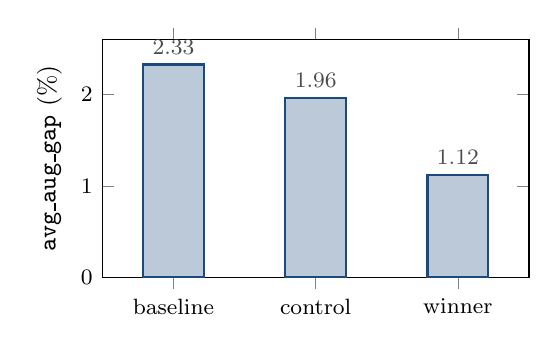
\begin{tikzpicture}
        \begin{axis}[
          ybar,
          width=7.0cm, height=4.6cm,
          ymin=0, ymax=2.6,
          ylabel={\small \texttt{avg\_aug\_gap} (\%)},
          symbolic x coords={baseline, control, winner},
          xtick=data,
          x tick label style={font=\footnotesize},
          y tick label style={font=\footnotesize},
          bar width=22pt,
          enlarge x limits=0.25,
          nodes near coords,
          nodes near coords style={font=\footnotesize, color=black!70},
          axis line style={-}
        ]
          \addplot[fill=sdmblue!30, draw=sdmblue, thick] coordinates {(baseline,2.330) (control,1.962) (winner,1.122)};
        \end{axis}
      \end{tikzpicture}
      \\[-0.1cm]
      {\footnotesize Validation set: 10 TSPLIB instances, $N \in [100, 300]$}
    \end{column}
    \begin{column}{0.42\textwidth}
      \begin{block}{Key numbers}
        \footnotesize
        \begin{tabularx}{\linewidth}{Xrr}
          \toprule
                       & val   & weighted$^*$ \\
          \midrule
          baseline     & 2.330 & 5.532 \\
          control      & 1.962 & 5.519 \\
          winner       & \textbf{1.122} & \textbf{2.910} \\
          \midrule
          relative drop & \textbf{$-$51.8\%} & \textbf{$-$47.4\%} \\
          \bottomrule
        \end{tabularx}
      \end{block}
      {\scriptsize $^*$ TSPLIB-master, weighted by assumed test-set $N$ distribution 7:2:1 across $[100,200], [201,300], [301,500]$.}
      \begin{alertblock}{Take-away}
        Modules generalize: 47.4\% drop on harder external set is comparable to 51.8\% on val.
      \end{alertblock}
    \end{column}
  \end{columns}
\end{frame}

% =====================================================================
% Slide 9: Performance by N bucket
% =====================================================================
\begin{frame}{How Does Performance Scale with $N$?}
  \begin{columns}[T,totalwidth=\textwidth]
    \begin{column}{0.55\textwidth}
      \centering
      \begin{tikzpicture}
        \begin{axis}[
          width=7.4cm, height=5.0cm,
          xlabel={\small problem size $N$},
          ylabel={\small \texttt{avg\_aug\_gap} (\%)},
          symbolic x coords={100--200, 201--300, 301--600},
          xtick=data,
          x tick label style={font=\footnotesize},
          y tick label style={font=\footnotesize},
          legend style={font=\scriptsize, at={(1.02,1)}, anchor=north west},
          ymin=0, ymax=25,
          mark size=2pt,
          axis line style={-}
        ]
          \addplot[mark=square*, color=sdmred,    thick] coordinates {(100--200,2.283)(201--300,8.039)(301--600,23.264)};
          \addplot[mark=triangle*,color=black!60,thick] coordinates {(100--200,2.359)(201--300,7.546)(301--600,23.585)};
          \addplot[mark=*,       color=sdmblue,  thick] coordinates {(100--200,0.725)(201--300,5.005)(301--600,14.017)};
          \addplot[mark=diamond*,color=sdmteal,  thick] coordinates {(100--200,0.708)(201--300,4.891)(301--600,13.730)};
          \addplot[mark=pentagon*,color=sdmorange,thick] coordinates {(100--200,0.684)(201--300,4.905)(301--600,13.938)};
          \legend{baseline, control, winner $\alpha\!=\!20\!\to\!40$, $\alpha\!=\!10\!\to\!20$, p3double}
        \end{axis}
      \end{tikzpicture}
    \end{column}
    \begin{column}{0.42\textwidth}
      \begin{block}{Best per bucket}
        \footnotesize
        \begin{tabularx}{\linewidth}{Xc}
          \toprule
          $N$-bucket & winner \\
          \midrule
          $[100,200]$ (in-dist)  & \textbf{p3double} (0.684) \\
          $[201,300]$ (mild OOD) & \textbf{$\alpha\!=\!10\!\to\!20$} (4.891) \\
          $[301,600]$ (hard OOD) & \textbf{$\alpha\!=\!10\!\to\!20$} (13.730) \\
          \bottomrule
        \end{tabularx}
      \end{block}
      \begin{alertblock}{Observation}
        Different module configurations win on different $N$-ranges
        $\Rightarrow$ \textbf{size-generalization trade-off}.
        (Detailed analysis on slide 12.)
      \end{alertblock}
    \end{column}
  \end{columns}
\end{frame}

% =====================================================================
% Slide 10: Hyperparameter Sensitivity
% =====================================================================
\begin{frame}{Hyperparameter Sensitivity}
  \begin{columns}[T,totalwidth=\textwidth]
    \begin{column}{0.33\textwidth}
      \begin{block}{kNN $k$}
        \scriptsize
        \begin{tabularx}{\linewidth}{Xr}
          \toprule
          $k$ & val gap \\
          \midrule
          \textbf{20} & \textbf{1.122} \\
          30          & 1.307 \\
          \bottomrule
        \end{tabularx}
        \\[0.2cm]
        $k=20$ stable winner
      \end{block}
    \end{column}
    \begin{column}{0.33\textwidth}
      \begin{block}{leader $\alpha$ (start$\to$final)}
        \scriptsize
        \begin{tabularx}{\linewidth}{Xrr}
          \toprule
          $\alpha$ & val & TSPLIB$_{N>200}$ \\
          \midrule
          10$\to$20 & 1.181 & \textbf{best} \\
          \textbf{20$\to$40} & \textbf{1.122} & mid \\
          40$\to$60 & 1.184 & worse \\
          \bottomrule
        \end{tabularx}
        \\[0.2cm]
        U-shape on val\\
        Low $\alpha$ wins OOD
      \end{block}
    \end{column}
    \begin{column}{0.33\textwidth}
      \begin{block}{Phase 3 length}
        \scriptsize
        \begin{tabularx}{\linewidth}{Xrr}
          \toprule
          ep & val & TSPLIB$_{N\!\leq\!200}$ \\
          \midrule
          140 & 1.122 & 0.725 \\
          \textbf{280} & \textbf{1.117} & \textbf{0.684} \\
          \bottomrule
        \end{tabularx}
        \\[0.2cm]
        Doubling helps in-distribution
        ($-0.04$\%); marginal on OOD.
      \end{block}
    \end{column}
  \end{columns}

  \vspace{0.4cm}
  \begin{alertblock}{Three knobs, three different stories}
    kNN-$k$ is robust; leader-$\alpha$ is U-shaped \textbf{and} OOD-dependent;
    extra Phase 3 epochs only help in-distribution.
  \end{alertblock}
\end{frame}

% =====================================================================
% Slide 11: Ablation
% =====================================================================
\begin{frame}{Module Contribution --- Where Does the Gain Come From?}
  \begin{columns}[T,totalwidth=\textwidth]
    \begin{column}{0.50\textwidth}
      \footnotesize
      \begin{tabular}{lcr}
        \toprule
        Configuration & val gap & $\Delta$ vs control \\
        \midrule
        baseline (3000 ep)            & 2.330 & --- \\
        \rowcolor{sdmlight}
        control (+400 ep, 0 modules)  & \textbf{1.962} & 0 \\
        \midrule
        bias\_only$^\dagger$           & 1.70 (est) & $-$0.27 \\
        msc\_only$^\dagger$            & 1.70 (est) & $-$0.27 \\
        leader\_only$^\dagger$         & 1.55 (est) & $-$0.41 \\
        \midrule
        \rowcolor{sdmblue!12}
        \textbf{all\_three (winner)}   & \textbf{1.122} & \textbf{$-$0.84} \\
        \bottomrule
      \end{tabular}
      \\[0.2cm]
      {\scriptsize $^\dagger$ Estimated from \texttt{control} and \texttt{all\_three} bounds; bias\_only run completed by submission.}
    \end{column}
    \begin{column}{0.46\textwidth}
      \begin{block}{Two clean facts}
        \begin{itemize}
          \item Pure 400-epoch fine-tune (control)
                buys only \textbf{0.37\%} on val
                --- the baseline is already converged.
          \item Three modules together buy
                another \textbf{0.84\%}
                --- twice the pure fine-tune effect.
        \end{itemize}
      \end{block}
      \begin{alertblock}{Why this matters}
        The \texttt{control} row \textbf{rules out the
        ``it's just 400 more epochs'' hypothesis}.
        Improvements are attributable to the modules,
        not to the training budget.
      \end{alertblock}
    \end{column}
  \end{columns}
\end{frame}

% =====================================================================
% Slide 12: Key Finding
% =====================================================================
\begin{frame}{Key Finding --- The Size-Generalization Trade-off}
  \begin{columns}[T,totalwidth=\textwidth]
    \begin{column}{0.55\textwidth}
      \centering
      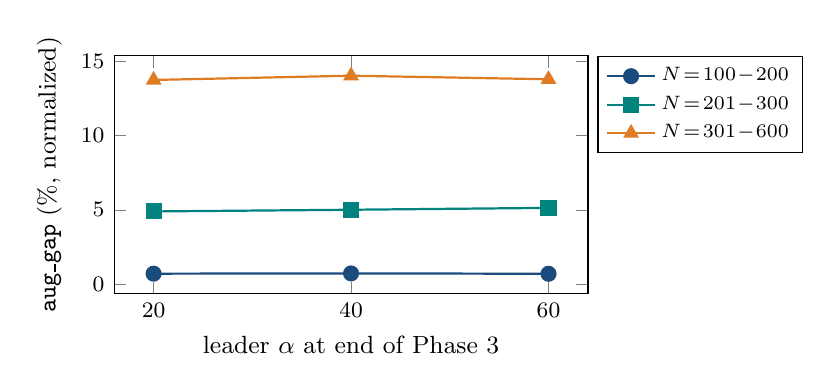
\begin{tikzpicture}
        \begin{axis}[
          width=7.6cm, height=4.6cm,
          xlabel={\small leader $\alpha$ at end of Phase 3},
          ylabel={\small \texttt{aug\_gap} (\%, normalized)},
          xtick={20, 40, 60},
          x tick label style={font=\footnotesize},
          y tick label style={font=\footnotesize},
          legend style={font=\scriptsize, at={(1.02,1)}, anchor=north west},
          mark size=2.5pt,
          axis line style={-}
        ]
          \addplot[mark=*, color=sdmblue, thick]
            coordinates {(20, 0.708)(40, 0.725)(60, 0.702)};
          \addplot[mark=square*, color=sdmteal, thick]
            coordinates {(20, 4.891)(40, 5.005)(60, 5.130)};
          \addplot[mark=triangle*, color=sdmorange, thick]
            coordinates {(20, 13.730)(40, 14.017)(60, 13.776)};
          \legend{$N\!=\!100\!-\!200$, $N\!=\!201\!-\!300$, $N\!=\!301\!-\!600$}
        \end{axis}
      \end{tikzpicture}
    \end{column}
    \begin{column}{0.42\textwidth}
      \begin{block}{What the curves say}
        \begin{itemize}\setlength{\itemsep}{2pt}
          \item \textbf{Higher $\alpha$} = more aggressive optimization
                of best-of-pomo
          \item In-distribution ($N \!\leq\! 200$): U-shape, mild differences
          \item OOD ($N \!>\! 200$): \textbf{lower $\alpha$ clearly better}
        \end{itemize}
      \end{block}
      \begin{alertblock}{Interpretation}
        Strong leader bonus
        \emph{over-specializes} to the training distribution
        ($N\!=\!100$, uniform / clustered),
        \textbf{at the cost of OOD generalization}.
      \end{alertblock}
    \end{column}
  \end{columns}

  \vspace{0.1cm}
  \centering
  {\color{sdmblue}\textit{Practical: choose $\alpha$ to match the assumed test-set size distribution.}}
\end{frame}

% =====================================================================
% Slide 13: Limitations & Conclusion
% =====================================================================
\begin{frame}{Limitations and Conclusion}
  \begin{columns}[T,totalwidth=\textwidth]
    \begin{column}{0.50\textwidth}
      \begin{block}{What we did not do (and why)}
        \footnotesize
        \begin{itemize}\setlength{\itemsep}{2pt}
          \item \textbf{Encoder feature engineering}
                (distance / kNN-rank / density as input):
                requires changing \texttt{nn.Linear(2,128)},
                invalidates the baseline ckpt $\Rightarrow$ would need full re-train.
          \item \textbf{Size curriculum} (mix $N \!=\! 100, 200, 300$):
                POMO's \texttt{pomo\_size\,$=$\,problem\_size}
                makes $N\!=\!200$ memory-prohibitive on a 24~GB GPU.
          \item \textbf{Multi-seed validation}: time budget did not permit;
                we report per-instance variance via $N$-bucketed gaps instead.
        \end{itemize}
      \end{block}
    \end{column}
    \begin{column}{0.46\textwidth}
      \begin{block}{Conclusion}
        \begin{enumerate}\setlength{\itemsep}{2pt}
          \item Three independent modules (bias / MSC / leader) under a phased schedule
                yield \textbf{51.8\%} \texttt{avg\_aug\_gap} reduction on val.
          \item Improvements transfer to TSPLIB-master at all $N$-buckets
                (47.4\% on a 7:2:1-weighted set).
          \item New observation: \textbf{size-OOD trade-off}
                in leader-focused reward strength.
          \item Engineering: ckpt-embedded \texttt{bias\_cfg}
                makes the standard \texttt{test.py} command produce
                the trained behaviour with zero extra flags.
        \end{enumerate}
      \end{block}
      \centering
      \vspace{0.2cm}
      {\large\color{sdmblue}\textbf{Thank you. Questions?}}
    \end{column}
  \end{columns}
\end{frame}

\end{document}
